\documentclass[10pt,twocolumn]{article}

\usepackage{fullpage}
\usepackage{times}
\usepackage{multirow}
\usepackage{arydshln}
\usepackage{amssymb,amsmath}
\usepackage{ifxetex,ifluatex}
\usepackage{fixltx2e} % provides \textsubscript
\ifnum 0\ifxetex 1\fi\ifluatex 1\fi=0 % if pdftex
  \usepackage[T1]{fontenc}
  \usepackage[utf8]{inputenc}
\else % if luatex or xelatex
  \ifxetex
    \usepackage{mathspec}
    \usepackage{xltxtra,xunicode}
  \else
    \usepackage{fontspec}
  \fi
  \defaultfontfeatures{Mapping=tex-text,Scale=MatchLowercase}
  \newcommand{\euro}{€}
\fi
% use upquote if available, for straight quotes in verbatim environments
\IfFileExists{upquote.sty}{\usepackage{upquote}}{}
% use microtype if available
\IfFileExists{microtype.sty}{%
\usepackage{microtype}
\UseMicrotypeSet[protrusion]{basicmath} % disable protrusion for tt fonts
}{}
%\usepackage{biblatex}
%\bibliography{paper}
\usepackage{graphicx}
\usepackage[small]{caption}
\usepackage{pstricks}
\makeatletter
\def\maxwidth{\ifdim\Gin@nat@width>\linewidth\linewidth\else\Gin@nat@width\fi}
\def\maxheight{\ifdim\Gin@nat@height>\textheight\textheight\else\Gin@nat@height\fi}
\makeatother
% Scale images if necessary, so that they will not overflow the page
% margins by default, and it is still possible to overwrite the defaults
% using explicit options in \includegraphics[width, height, ...]{}
\setkeys{Gin}{width=\maxwidth,height=\maxheight,keepaspectratio}
\ifxetex
  \usepackage[setpagesize=false, % page size defined by xetex
              unicode=false, % unicode breaks when used with xetex
              xetex]{hyperref}
\else
  \usepackage[unicode=true]{hyperref}
\fi
\hypersetup{breaklinks=true,
            bookmarks=true,
            pdfauthor={},
            pdftitle={Malacology: A Programmable Storage System Built on Ceph},
            colorlinks=true,
            citecolor=blue,
            urlcolor=blue,
            linkcolor=black,
            pdfborder={0 0 0}}
\urlstyle{same}  % don't use monospace font for urls
\setlength{\parindent}{0pt}
\setlength{\parskip}{6pt plus 2pt minus 1pt}
\setlength{\emergencystretch}{3em}  % prevent overfull lines
\setcounter{secnumdepth}{5}

\title{Malacology: A Programmable Storage System Built on Ceph}
\author{Paper \# 123}
\date{}
\begin{document}

\maketitle

\begin{abstract}
Storage systems are caught between rapidly changing data processing systems and
the increasing speed of storage devices. This puts tremendous pressure on
storage systems to adapt both in terms of their interfaces and their
performance. But adapting storage systems can be difficult because unprincipled
changes might jeopardize years of code-hardening and performance optimization
efforts that were necessary for users to entrust their data to the storage
system.  We introduce  Malacology, a prototype programmable storage system to
explore how existing abstractions of common services found in storage systems
can be leveraged to address new data processing systems and the increasing
speed of storage devices. This approach allows unprecedented flexibility for
storage systems to evolve without sacrificing the robustness of its
code-hardened subsystems.  We illustrate the advantages and challenges of
programmability by constructing two services out of existing abstractions: a
file system metadata load balancer and a high-performance distributed shared-log
that leverages flash devices.  RESULTS
\end{abstract}

\section{Introduction}\label{introduction}

A storage system implements abstractions designed to persistently store
data and must exhibit a high level of correctness to prevent data loss.
Storage systems have evolved around storage devices that often were
orders of magnitude slower than CPU and memory and therefore can
dominate overall performance if not used carefully. Over the last few
decades members of the storage systems community have developed
ingenious strategies to meet correctness requirements while somewhat
hiding the latency of traditional storage media. To avoid lock-in by a
particular vendor, users of storage systems have preferred systems with
highly standardized APIs and lowest common denominator abstract data
types such as blocks of bytes and byte stream files.

A number of recent developments are disrupting traditional storage
systems: (1) the falling prices of flash storage and the availability of
new types of non-volatile memory that are orders of magnitude faster
than traditional spinning media are moving overall performance
bottlenecks away from storage devices to CPUs and networking, and
pressure storage systems to shorten their code paths and incorporate new
optimizations; (2) demand for managing structured data and flexible
consistency semantics at scale pressure big data processing systems to
use storage abstractions that can meet these demands; and (3)
production-quality scalable storage systems available as open source
software have established and are continuing to establish new, \emph{de
facto} API standards at a faster pace than traditional standards bodies.

These three trends put evolutionary pressure on storage systems and
raise the question whether there are principles that storage systems
designers can follow to evolve storage systems efficiently and without
jeopardizing years of code-hardening and performance optimization
efforts that are important for users to continue to entrust their data
to the storage system.

In this paper we investigate an approach that focusses on generalizing
existing storage system resources, services, and abstractions that in
generalized form can be used to \emph{program} new services. By doing so
one can reuse subsystems and their optimizations and leverage their
established correctness, robustness, and efficiency. We will refer to
this programmability as \emph{programmable storage}, which differs from
\emph{active storage} (the injection and execution of arbitrary code in
a storage system) and \emph{software-defined storage} (the control of
thin-provisioning of storage).

To illustrate the benefits and challenges of this approach we examine
the programmability of Ceph~\cite{weil_ceph_2006}, the increasingly
popular, production-level open-source distributed storage system.
Something of a storage swiss army knife, Ceph supports file, block, and
object interfaces simultaneously in a single cluster. Ceph's Reliable Autonomous Distributed Object Storage (RADOS) system is a cluster of storage
devices (OSDs) that provide Ceph with data durability and integrity
using replication, erasure-coding, and scrubbing~\cite{weil_rados_2007}. 
% By introducing
% programmability concepts into Ceph, we can build new services by
% carefully exposing internal storage services to applications.

\begin{figure}[htbp]
\centering
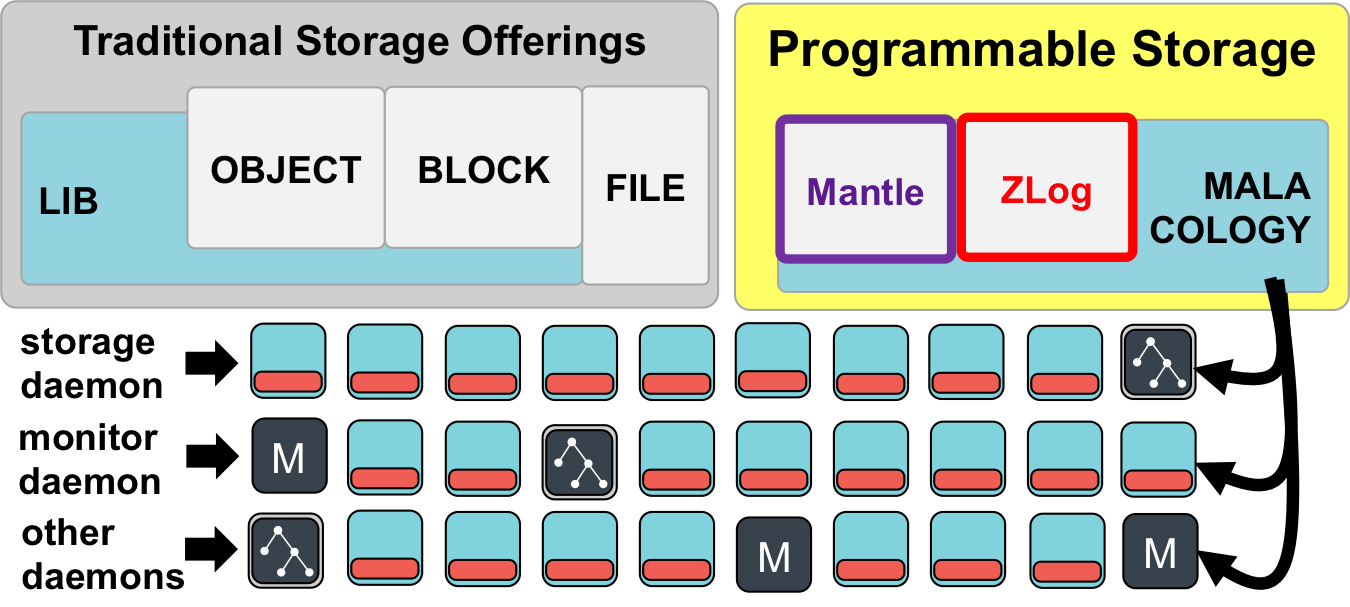
\includegraphics{figures/overview.png}
\caption{A Ceph installation consists of a cluster running mostly
storage daemons (OSDs) to ensure data durability, a few monitor daemons
(MONs) to reach consensus of the cluster state and to ensure its
consistent versioning, and a few metadata service daemons (MDSs) for
scalable metadata service. Ceph's APIs include object, block, file
abstractions. Malacology enables the programmability of these
abstractions and services. To illustrate Malacology we implement two
services on Ceph, Zlog and Mantle, by programming Ceph's durability,
consistent versioning, consensus, and metadata subsystems.
\label{fig:overview}}
\end{figure}

For example, a Ceph cluster contains a small number of
monitoring nodes (MONs) that use PAXOS to maintain a consistent view of
system-wide metadata such as data distribution parameters and cluster
membership. The data distribution metadata maintained by
the cluster monitors is used by RADOS servers and clients to provide
consistent reads and writes, and both RADOS and the monitoring services
are used by a cluster of file system metadata servers that provide POSIX
semantics using sophisticated indexing and distributed locking services.
We contend that re-using and re-purposing these code-hardened subsystems
is paramount to successfully adapting storage systems to new APIs and
new storage devices without losing the benefits from years of
code-hardening work.

To illustrate the benefits and challenges of this approach we have
designed and evaluated Malacology, a programmable storage system for
constructing new functionality by re-purposing existing subsystem
abstractions contained in Ceph. We build the framework on Ceph by
leveraging a broad spectrum of existing services, including distributed
locking and caching services provides by MDSs, durability and logical
storage devices provided by RADOS, and propogation of consistent cluster
state provided by the monitoring service (see \ref{fig:overview}). As we will show in this paper, this framework is expressive enough to provide the
functionality necessary for implementing new services. Our contributions
are:

\paragraph{}

\begin{itemize}
\itemsep1pt\parskip0pt\parsep0pt
\item A programmable storage system implementation that re-uses and extends existing abstractions. It includes:

  \begin{enumerate}
  \def\labelenumi{\arabic{enumi}.}
  \itemsep1pt\parskip0pt\parsep0pt
  \item
    Extending file system metadata by a new type of ``sequencer'' inode that together with Ceph's capability subsystem implements high-performance, non-durable access serialization
  \item
    Re-using Ceph's PAXOS-based consensus infrastructure for versioning of metadata service load-balancing policies
  \item
    Re-using storage objects for persisting policies
  \item
    Extending object interface classes for new logical storage/metadata devices
  \end{enumerate}
\item
  Two example implementations and evaluations for feasibility of services that use this framework

  \begin{enumerate}
  \def\labelenumi{\arabic{enumi}.}
  \itemsep1pt\parskip0pt\parsep0pt
  \item
    A high-performance distributed shared log service called Zlog which is based on CORFU~\cite{balakrishnan_corfu_2012}
  \item
    A re-implementation of the programmable Mantle metadata load balancing service using Malacology~\cite{sevilla:sc15-mantle}
  \item 
    An application of the Mantle metadata load balancing service to manage the placement of new sequencer inodes.
  \end{enumerate}
\end{itemize}

First, we describe existing techniques for bridging the gap between the
performance of storage systems and the requirements of applications
(\S\ref{problem}). Next, we discuss the ``distributed systems'' inspired
abstractions employed by Ceph (\S\ref{background}) and allude to their
re-usability as components in other services. The next section
enumerates the abstractions that Malacology exposes in the
implementation section (\S\ref{implementation}). We then show how we use
Malacology to synthesize entirely new storage services on an existing
system through configuration and small changes (\S\ref{services}). We
conclude by evaluating real-world use cases (\S\ref{evaluation}).

\section{Highly Tailored and Application-Specifc Storage
Systems}\label{highly-tailored-and-application-specifc-storage-systems}

\label{problem}

A consequence of complicated data management requirements and faster storage
devices is that storage systems may fail to meet the needs of applications.
Application workarounds for meeting performance goals roughly fall into one of
three categories: ``bolt-on'' services, application changes, and changes to
the storage system itself.

\subsection{\texorpdfstring{``Bolt-on''
services}{Bolt-on services}}\label{bolt-on-services}

So called ``bolt-on'' services are third-party solutions integrated into a
system to provide functionality and improve performance for common use-cases
(e.g. a metadata service). The introduction of additional services may provide
simplicity and performance enhancements, but ``bolt-on'' services often
duplicate functionality, unnecessarily increasing the likelihood of bugs or
introducing unpredictable performance problems. For example, we are developing
a high-performance distributed shared-log on Ceph called ZLog, based on the
CORFU protocol~\cite{corfu}. Serialization at high-performance is achieved using a
``sequencer'' service that maintains a volatile, in-memory counter used to assign a log
position to each client that appends to the log. One option for building
a distributed log is to use PAXOS, or an out-of-the-box solution such as
Zookeeper. However, these systems adhere to the pre-coneived notions of
storage, namely that data is safe from data loss, which is exactly the feature
that causes traditional approaches to run at significantly reduced speed.

\subsection{Application Changes}\label{application-changes}

The second approach that applications may use to adapt to a storage system
limitation is to
extend the responsibility of the application. This means changing the
application itself by adding more data management intelligence or
using domain-specific middleware (e.g., a new data layout). For instance, an
application may be changed to exploit data locality or I/O
parallelism in a distributed storage system.

For example, SciHadoop~\cite{buck:hpc2011-scihadoop,buck:sc2013-scidr} changes both the Hadoop
application and the Hadoop framework itself to leverage the structure of
scientific data (3D array-based data, more specifically) to increase
performance, locality, and the number of early results. This is not a
bad proposition, but creates a coupling that is highly tied to the
underlying physical properties of the system, making it difficult to
adapt to future changes at the storage system level.

\subsection{Storage System Changes}\label{storage-changes}

When these two approaches fail to meet the needs of the application,
developers turn their attention to the storage system itself.
Traditionally, storage system behaviour can be altered using two
techniques: tuning the system or introducing changes to the system. The
difficulty of both of these approaches has given rise to a third
technique called active storage.

\subsubsection{Tuning}\label{tuning}

Tuning large and complicated systems is difficult because of the number
of parameters (e.g., Hadoop 2.7.1 has 210 tunables) and because the
tunables are difficult to understand or quantify (e.g., Ceph tunables~\cite{sevilla:sc15-mantle}). To succesfully tune the system, a
developer must have domain and system specific knowledge. Without this
intimate knowledge, the tuning turns into somewhat of a black art, where
the only way to figure out the best settings is trial and error.

Auto-tuning techniques attempt to find a good solution among a huge space of
available system configurations. However, in practice auto-tuning is limited
to only the configuration tunables that the storage system exposes and can be
overwhelmed with too many parameters.  For instance, auto-tuning may be
capable of identifying instances in which new data layouts would benefit a
workload, but unless the system can provide such a transformation, the option
is left off the table.  Starfish~\cite{herodotou:cidr2011-starfish} made
an attempt of this for Hadoop but this technique would need to severely limit
the space of parameters in order to feasible, similar to the approach used in~\cite{behzad:sc2013-autotuning}.

\subsubsection{Software Changes}\label{software-changes}

As a last resort, the application developer can alter the storage system
itself. In the best case a developer is using an open-source system in which
case one must become familiar with often enormous code-bases before being able
to make changes, but then face the task of approaching a community to
integrate changes, or be forced to maintain an in-house version and risk
maintaining features that become incompatible.  A successful example of this
is the work that focused on HDFS scalability for metadata-intensive workloads~\cite{shvachko_hdfs_2010}. This has lead to modifications to its
architecture or API~\cite{balmin:sigmod2012-clydesdale} to improve
performance.

Alternatively, some systems have formal support for introducing additional
functionality, often in the form of a plugin infrastructure. Ceph provides the
ability to create domain-specific logical object interfaces by composing
existing interfaces. These interfaces are written in C++ and are statically
loaded into the system. An example usage may be to atomically combine a
``write'' with an index update to create a content-addressable object
interface.

\if{false}
As an example use-case, ZLog needs to
store metadata information with each object so for each operation, it
checks the epoch value and write capability (2 metadata reads) and
writes the index (metadata write).
\fi

Figure 1 shows the throughput
(\emph{y} axis) over time (\emph{x} axis) of two OSD implementations for
storing metadata: in the header of the byte stream (data) vs.~in the
object extended attributes (XATTR). The speed for appending data without
any metadata operations (data raw) is also shown as a baseline for
comparison. For append-heavy workloads storing metadata as a header in
the data performs about 1.5x better than storing metadata as an extended
attribute.

\begin{figure}[htbp]
\centering
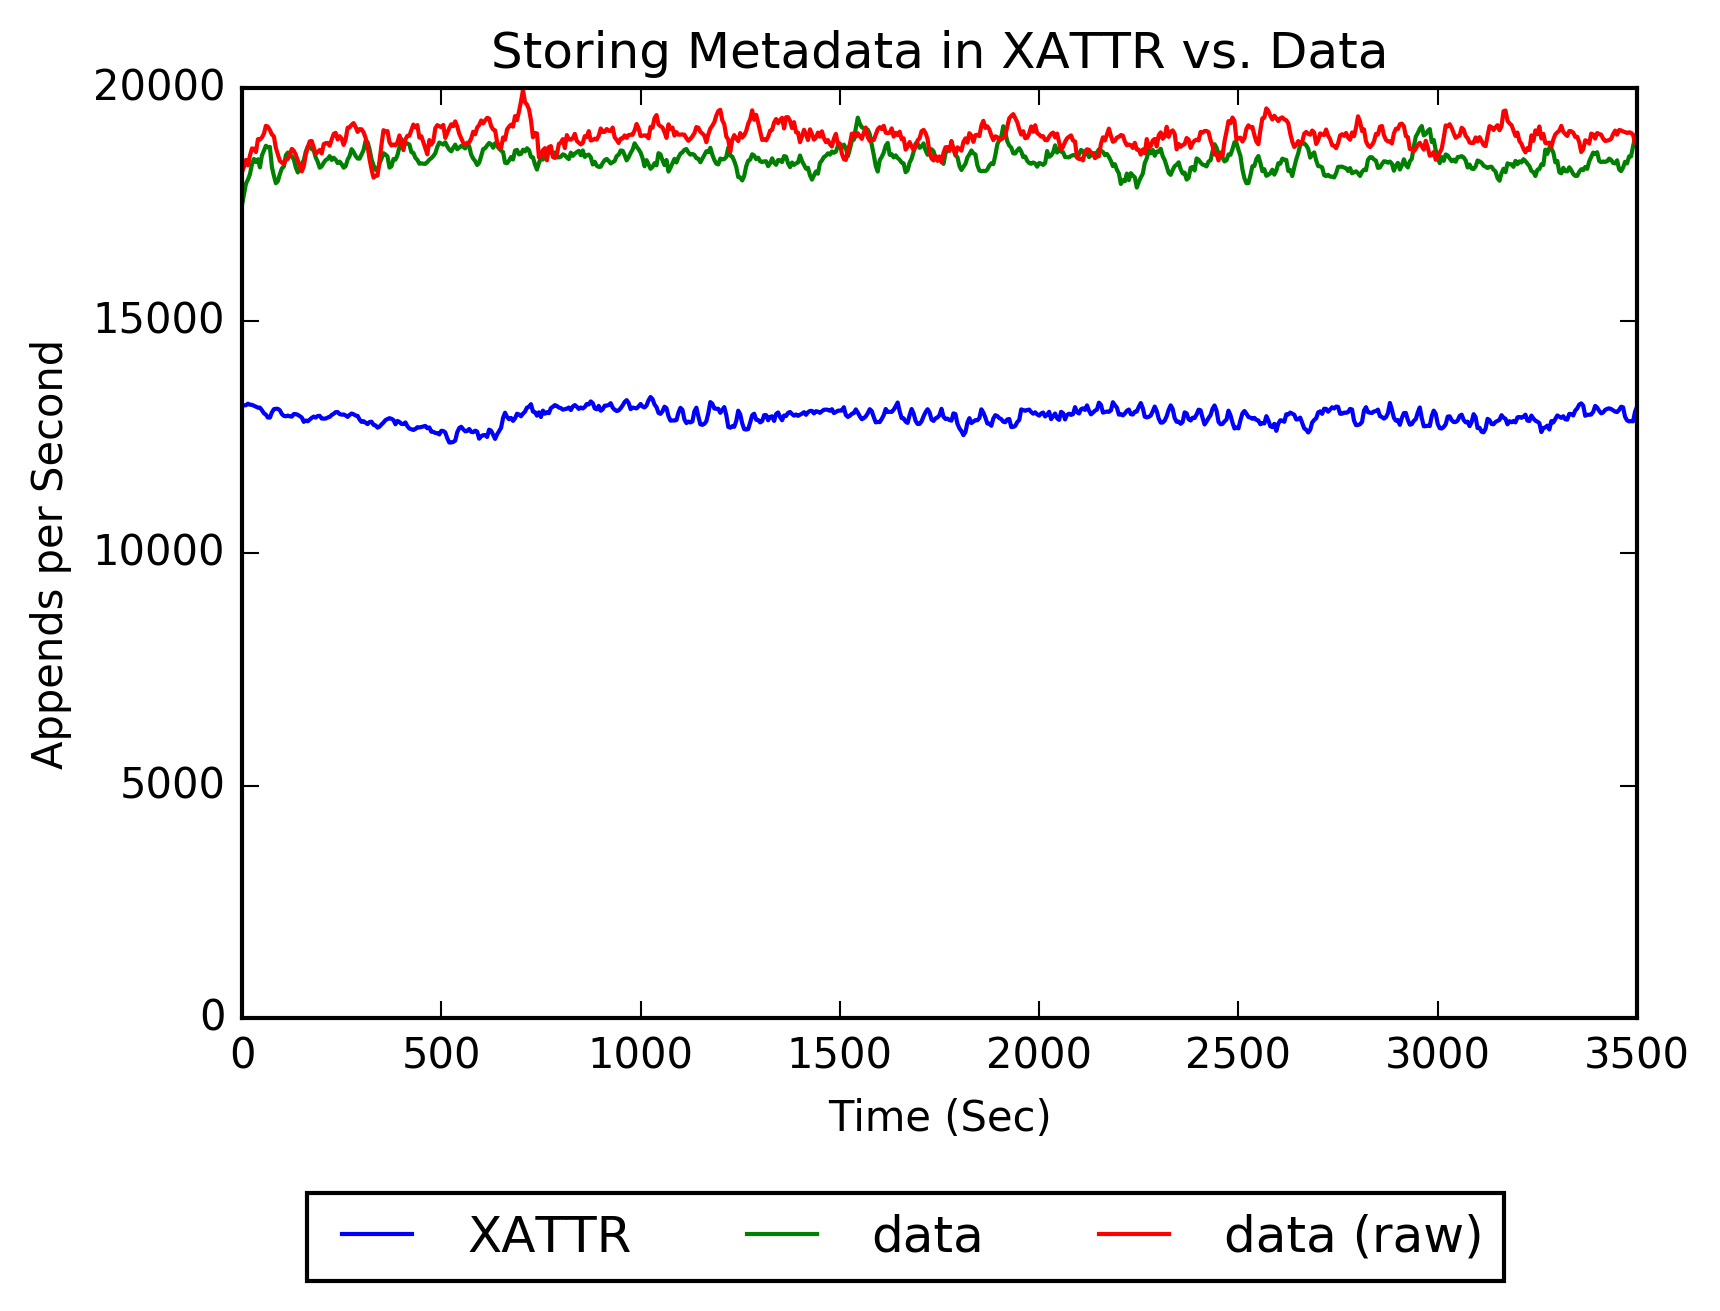
\includegraphics{figures/cls_xattr-vs-data.png}
\caption{{[}\href{https://github.com/michaelsevilla/malacology-popper/blob/master/experiments/figure1/visualize.ipynb}{source}{]}
When appending data to objects, the object class that stores metadata in
a header in the data byte stream (data) performs 1.5x better than the
object class that stores metdata in the extended attributes of the
object (XATTR); it is almost as fast as appending data without updating
metadata (data raw).}
\end{figure}

The object interface facility provided by Ceph is more than an
a proof-of-concept active storage implementation.  Figure
\ref{fig:obj-int-dev-growth} shows a dramatic growth in the production use of
domain-specific interfaces in the Ceph community since 2010.  What is most
remarkable is that this trend contradicts the notion that API changes are a
burden for users.
Rather it appears that a gap in existing interfaces are
being addressed through programmability. In fact, Table~\ref{table:objclasses}
categorizes existing interfaces and we clearly see a trend towards reusable
services.

\begin{figure}[ht]
\centering
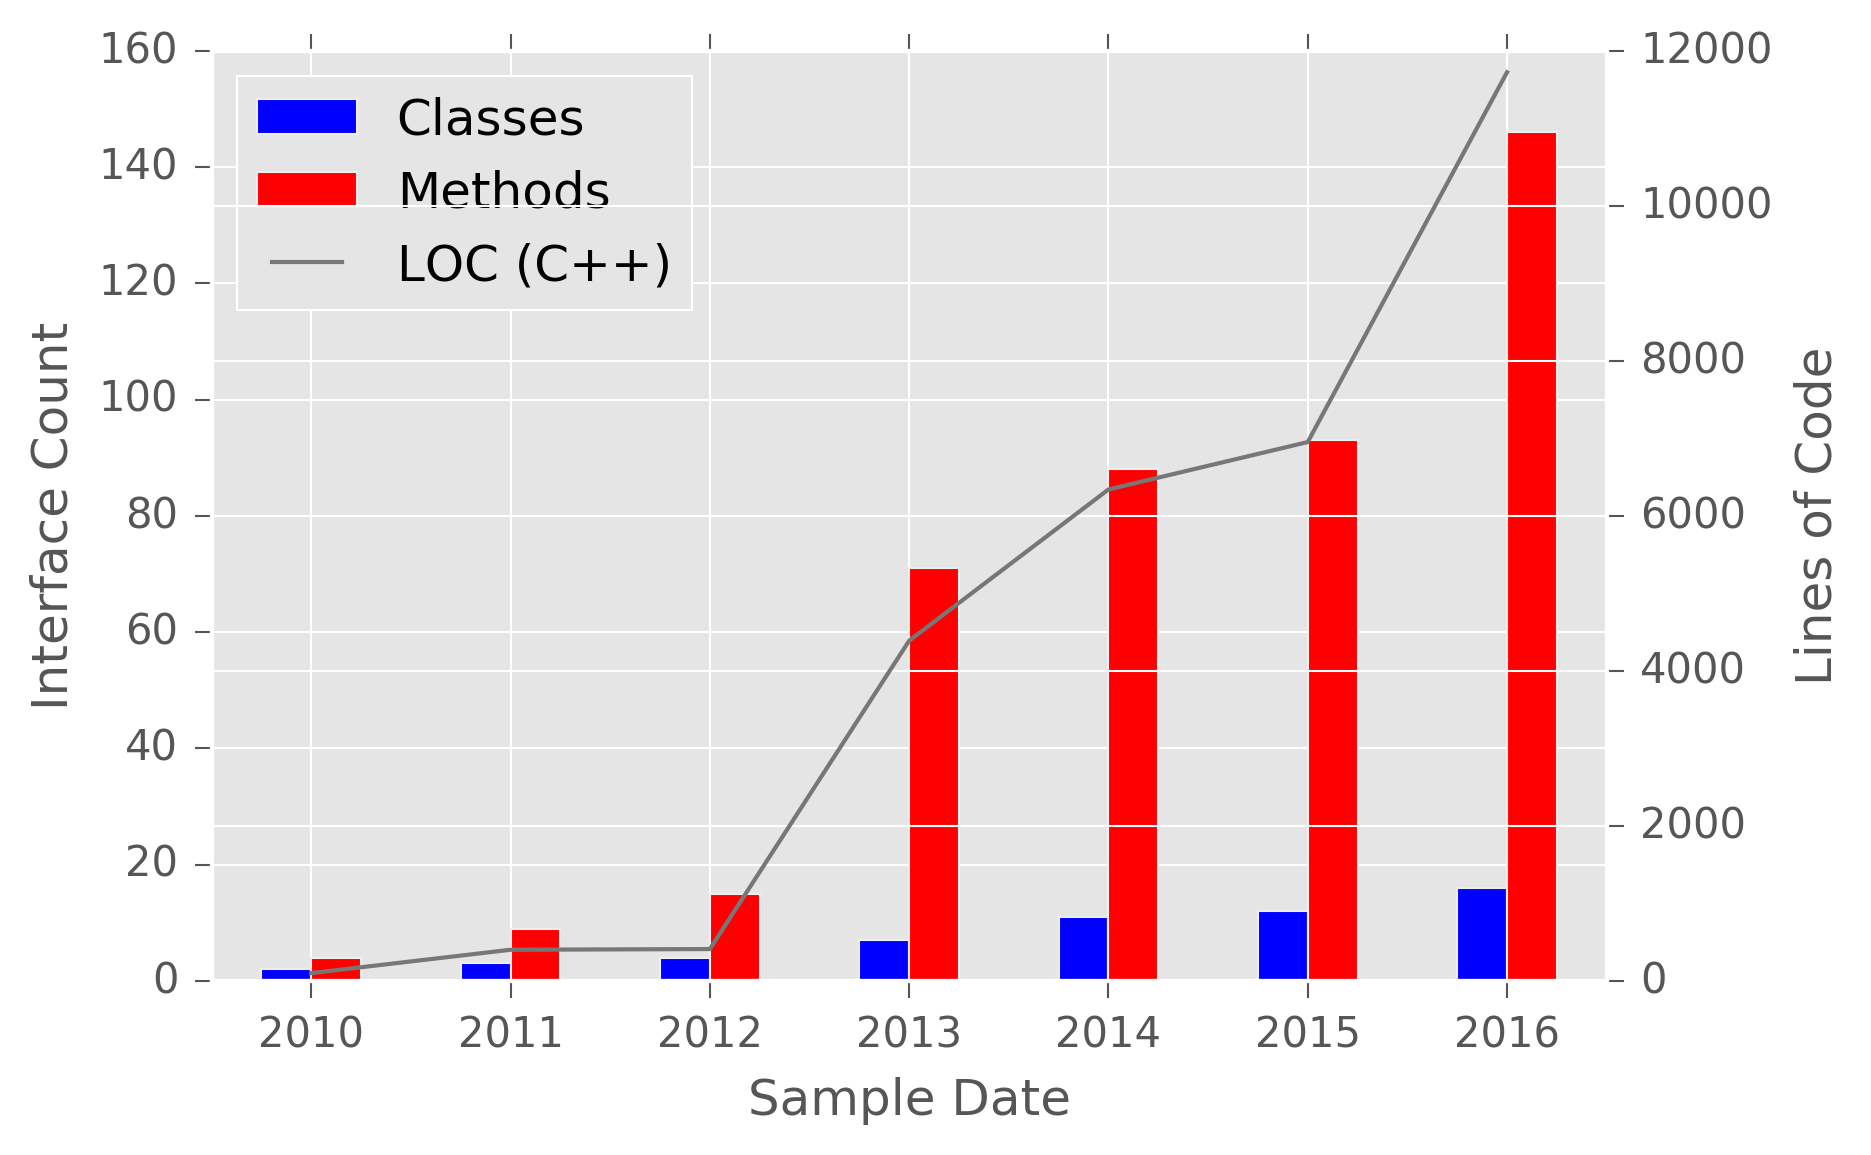
\includegraphics{figures/obj-int-dev-growth.png}
\caption{Since 2010, the growth in the number of co-designed object
storage interfaces in Ceph has been accelerating. This plot is the
number of object classes (a group of interfaces), and the total number
of methods (the actual API end-points).\label{fig:obj-int-dev-growth}}
\end{figure}

\begin{table}[ht]
\centering
  \begin{tabular}{l|l|l}
    Category & Specialization& \# \\ \hline
    \multirow{2}{*}{Locking} & Shared & \multirow{2}{*}{6} \\
                             & Exclusive & \\ \hdashline
    \multirow{3}{*}{Logging} & Replica & 3 \\
                             & State & 4 \\
                             & Timestamped & 4 \\ \hdashline
    \multirow{4}{*}{Metadata Managment} 
                             & RADOS Block Device  & 37 \\
                             & RADOS Gatway & 27 \\
                             & User & 5 \\
                             & Version & 5 \\ \hdashline
    Garbage Collection       & Reference Counting & 4 \\
\end{tabular}
\caption{A variety of RADOS object storage classes exist to expose interfaces
    to applications. \# is the number of methods that use these categories.
}
\label{table:objclasses}
\end{table}

\if{false}
\begin{figure}[htbp]
\centering
\includegraphics{figures/obj-int-dev-churn.png}
\caption{Source code changes over time indicate the dynamic interface
development will need to support a high frequency of interface churn.
Each dot represents a Ceph commit with a corresponding number of lines
of code changed. \label{fig:obj-int-dev-churn}}
\end{figure}
\fi

The popularity of the active storage component of Ceph hint at three
trends in the Ceph community: (1) increasingly, the default
algorithms/tunables of the storage system are insufficient for the
application's performance goals, (2) programmers are becoming more aware
of their application's behavior, and (3) programmers know how to manage
resources to improve performance. Programmers gravitate towards object
interfaces because it gives them ability to tell the storage system
about their application: if it is CPU or IO bound, if it has locality,
if its size has the potential to overload a single proxy node, etc. The
programmers know what the problem is and how to solve it, but until
object interfaces, had no way to tell the storage system how to handle
their data.

These implementations use the active storage interfaces in Ceph. We
refer to this as \emph{storage programmability} which is a method by
which an application communicates its requirements to the storage system
in a way that allows the application to realize a new behavior without
sacrificing the correctness of the underlying system. This evaluation
and resulting implementation would have been a burden without object
classes.

\section{Re-Usable Components in
Ceph}\label{re-usable-components-in-ceph}

\label{background}

Ceph is a production-quality distributed system and in this section we
touch on some of the subsystems it uses to provide a general-purpose
storage system. In the next section, we describe how we leverage these
subsystems to build new services.

\subsection{Durability}\label{durability}

Ceph provides storage by striping and replicating data across RADOS~\cite{weil_rados_2007}, the reliable distributed object store. RADOS
uses many techniques to ensure that data is not corrupted or lost, such
as erasure coding, replication, and data scrubbing. Furthermore, many of
these techniques try to be autonomous so that work is distributed across
the cluster. For example, when placement groups change the OSDs
rebalance and re-shard data in the background in a process called
placement group splitting.

\subsection{Consistency/Versioning of Cluster
State}\label{consistencyversioning-of-cluster-state}

Ceph needs to keep track of cluster state and it does this with separate
``services'': client authentication, logging, MDS maps, MON maps, OSD
maps and placement group (PG) maps. These services are all managed in
the MONs and they all talk to a PAXOS instance; this PAXOS instance goes
and talks to other PAXOS instances on other MONs so that they can all
agree on the correct version of the service; essentially they reach an
agreement about what the state of the cluster is.

\subsection{Active Storage}\label{active-storage}

Active storage attempts to push computation closer to the data by
exposing interfaces to execute code remotely. For example, the storage
server could process data before sending data over the network or
sorting it. The active storage component in Ceph is called ``object
interface classes'' (or \texttt{cls} for short). The Ceph object
interface classes can be loaded at runtime and customized with
user-defined functionality. The basic idea is shown in
Figure\textasciitilde{}\ref{fig:object-interfaces}, where the
\texttt{libcls\_md5.so} shared library performs the MD5 hash on an
object at the oSD instead of transferring data over the network. This
ability to carry out arbitrary operations on objects stored on OSDs
helps applications improve performance by optimizing things like network
round trips, data movement, and remote resources which may be idle.

Object storage interfaces are compiled into shared libraries and loaded
into a running OSD daemon using \texttt{dlopen()}. Because the shared
library has to link against symbols found in the running executable, the
interfaces are stored on the local file systems of each OSD so they can
be versioned and distributed alongside the same Ceph binaries. This
policy is for safety, since the OSDs could be on different distros that
provide different versioning capabilities. Also, this approach allows
bug fixes to co-evolve with the rest of the Ceph installation.

Although customizable OSD interfaces are powerful, the current
implementation has drawbacks. OSD interfaces are written in C/C++ and
compiled into a shared library, so the developer must account for
different target architectures. Second, C/C++ provides more
functionality than is necessary since the snippets of interface code
mainly set policies and perform simple operations. Finally, developing
these interfaces in C/C++ has high overhead. The developer must learn
how the OSD dynamically loads the shared libraries (\emph{e.g.}, OSDs
rely on a strict naming convention to find shared libraries), how to get
their interfaces compiled using the Ceph \texttt{make} system, and how
to debug issues that are not related to their specific interface
(\emph{e.g.}, the OSD cannot find the shared library) - this learning
curve is unacceptable for non-Ceph developers, especially since most
interfaces are one-off solutions specific to their applications.

Ceph has a whole infrastructure for getting dynamic code into the OSD.
The \texttt{ClassHandler} class safely opens object interfaces, executes
commands defined by the shared library, and fails gracefully with
helpful errors if anything goes wrong. Instead of injecting strings
directly into Ceph (like we did with the original Mantle
implementation), the \texttt{ClassHandler} class safely opens shared
code, even code with dependencies that are not in Ceph itself (e.g.,
Lua). With the \texttt{ClassHandler}, we get the safety and robustness
of loading dynamic code, the ease of transferring state between object
interfaces and the oSD internals, integration with testing and
correctness suites, and \texttt{struct}s for interface data and
handlers.

While we consider active storage to be an excellent example of
programmability, what separates our proposal from previous work is the
observation that so much \emph{more} of the storage system can be reused
to construct advanced, domain-specific interfaces.

\section{Malacology Implementation}\label{malacology-implementation}

\label{implementation}

To enable the programmability of Ceph subsystems, Malacology relies
heavily on interface classes for introducing new functionality into the
MDSs and OSDs. Malacology introduces 3 components to manage
object/metadata interfaces:

\begin{enumerate}
\def\labelenumi{\arabic{enumi}.}
\item
  additional interface hooks and classes for OSDs and MDSs using the
  existing Ceph \texttt{cls} infrastructure
\item
  durable interface classes using the Ceph object store
\item
  versioned and consistent interfaces using Ceph's consensus service
\end{enumerate}

In the following section, we will discuss the existing Ceph
infrastructure and the changes necessary for Malacology. Our focus will
be to demonstrate the viability and usefulness of the Malacology
appraoch with example implementations that due to limited time for the
submission of this paper are not necessarily fully optimized.

\subsection{Additional Interface Hooks and
Classes}\label{additional-interface-hooks-and-classes}

Malacology adds new hooks to Ceph and a new interface class for both the
MDS and OSD that uses Lua~\cite{ierusalimschy:lua15,ierusalimschy:spe96}. Our
framework has added a mechanism for defining and running object and
metadata balancer classes using Lua. Our Lua bindings expose functions
and symbols both ways; the host program can call functions defined in
Lua and the Lua scripts can call functions defined in native C++. These
bindings are merged upstream. We choose Lua for 4 reasons: performance,
portabability, size, and and security.

Lua is a fast scripting language. It was designed to be an embedded
language and the LuaJIT virtual machines boasts near-native performance~\cite{pall:luajit15,grawinkel_pdsw12}. Lua is frequently
used in game engines to set policies but we use it here because most of
the user-defined object classes in Ceph are policies as well (see
\S\ref{table:objclasses}). Separating policy from mechanism is a driving
factor in using Lua.

\begin{figure}[htbp]
\centering
\includegraphics{figures/programmability-framework.png}
\caption{Clients add functionality by injecting Lua scripts with a new
monitor (M) command. After the ``proposal'' (using PAXOS terminology) is
accepted by the cluster of monitors, the script is redundantly and
consistently distributed to OSDs. \label{fig:programmability-framework}}
\end{figure}

For object interfaces, clients send Lua classes to the OSD and then they
can invoke operations in that class remotely on the OSD. In reality,
this feature is a statically loaded object class written in C/C++ that
runs dynamically defined object interfaces, where clients access the
classes using an \texttt{exec()} wrapper. Although sending the class
with each client request is stateless (which has its own set of nice
features), it is costly for network bandwidth and difficult to organize
at the application level. Also, while the execute wrapper simplifies the
implementation, it burdens the applications, since they need to be
recompiled to use the \texttt{exec()} function.

Our framework has a mechanism for defining and running object and
metadata balancer classes with scripting. Scripting is useful in large
systems for 3 reasons: - accelerates deployment: tweaking policies, like
changing a threshold or metric calculation, does not require a full
recompile or system start-up. - transparency: if the bindings carefully
expose the correct metrics and functions, the user does not need to
learn the internal functions, variables, or types of the system. -
portability: scripts can be exchanged across platforms and system
versions without compatibility issues.

This effectively decouples policy from mechanism, which helps future
designers explore trade-offs and isolates policy development from
code-hardened systems. Decoupling policy mechanism is not a new
technique but designing the storage system with programmability as a
first-class citizen is credits policy/mechanism separation as the
biggest reason for the success of the block allocation mechanisms in the
Fast File System~\cite{mckusick:fast2015-FFS} yet there
are no mechanisms for transparently exposing and modifying the
underlying logic in modern file systems.

Malacology has Lua bindings that expose functions and symbols both ways;
the host program can call functions defined in Lua and the Lua scripts
can call functions defined in native C++. These bindings are merged
upstream. We choose Lua for 4 reasons: performance, portabability, size,
and security.

\subsubsection{Using Lua}\label{using-lua}

Lua is a performs well as an embeddable scripting language. Although it
is an interpreted language, the bindings are designed to make the
exchange of variables and functions amongst languages straightforward.
The LuaJIT virtual machine boasts near-native performance, making it a
logical choice for scriptability frameworks in systems research~\cite{neto:dls14-luaos}. In storage systems, it has been effectively
used both on \cite{grawinkel:pdsw2012-lua,watkins2013:bdmc13-in-vivo} and off
\cite{sevilla:sc15-mantle} the critical path, where performance is
important. Lua is frequently used in game engines to set policies but we
use it here because most of the user-defined classes in Ceph are
policies as well! We do not want to provide specific implementations,
like pulling data from objects or transferring them over the network,
but instead strive to say \emph{what to do} with the data once we have
it. Separating policy from mechanism is a driving factor in using Lua.

Because Lua is interpreted, it is also portable. The portability allows
functions to be shipped around the cluster without having to compile or
reason about compatibility issues. Traditionally, intefaces are written
in C/C++, so they must be compiled into shared libraries before being
injected into the daemon at runtime. Shared libraries need to be
compiled on the host they will be run on to accomodate different
architectures and dependendencies. Embedding the Lua interpretator, on
the other hand, gives us the flexbility to store the actual Lua code in
other places, like RADOS, so we can enjoy all the other properties
provided by that particular back-end.

The other two advantages, that Lua leaves a small memory footprint and
that is is secure, are discussed at length in~\cite{ierusalimschy_programming_2006,neto:dls14-luaos}. In short, Lua
provides relatively robust sandbox capabilities for protecting the
system against some malicious cases, but does not protect the system
from poor policies. Since Malacology does not use these features (yet),
we will avoid discussion here.

\subsubsection{Generalizing the Lua VM}\label{generalizing-the-lua-vm}

We generalize the Lua VM since it will be used in both the OSD and MDS.
We put the core sandbox wrapper for the Lua object interface in a common
directory in Ceph and link against it. This core Lua wrapper contains
just the dependencies, symbols, and functions, need to run the Lua VM.
Some of these functions include \texttt{clslua\_log()} for transferring
logs to the daemon logs and \texttt{clslua\_pcall()} for calling Lua
functions.

Dependencies, symbols, and functions specific to the object or balancer
interface are put in the \texttt{cls} or \texttt{bal} directories,
respectively. For example, the Lua object interface uses functions that
have placement group filters, cryptography functions, and object
metadata (\emph{it i.e.} \texttt{cxx\_omap\_getvals()}, object data,
object extended attributes, and object versions -- all these are
dependencies, symbols, and functions are part of the OSD process but not
the MDS process. As a result, we put interface code that uses these in
\texttt{cls} directory. With this scheme, The OSD will \texttt{dlopen()}
the shared library created by Lua object interface shared library while
the MDS will \texttt{dlopen()} the Lua balancer interface shared
library; both shared libraries will the Lua core.

Both the object and balancer interfaces define functions and attach them
to the core Lua sandbox. For example, the Lua object storage interface
class attaches data, extended attribute, object map, and object version
functions, to the the Lua core functions; the exact functions are shown
in Listing\textasciitilde{}\ref{lst:attach_functions}. The advantages of
this is that we avoid duplicating code, we provide a framework for
putting Lua code in other parts of the system, and we remove components
and APIs that are too integrated with the OSD.

\subsubsection{Generalizing the Class
Handler}\label{generalizing-the-class-handler}

Our framework can also load Lua interfaces from the local file system --
the same technique as the C/C++ object interfaces. First, the OSD looks
for C/C++ shared library. If the OSD cannot find the file, it looks for
a Lua script of the same name. The script is read into a string of the
C++ object class; this string is later forwarded to the native Lua
class. When a requests comes in, the method name is passed with the
\texttt{exec()} function and the corresponding function in the Lua class
is called. Now clients need to only send their Lua object class once and
the OSDs will store them locally. Also, clients can execute any Lua
handler they want.

\subsection{Storing Interfaces in
RADOS}\label{storing-interfaces-in-rados}

For balancer interfaces, clients put balancers into RADOS and the CephFS
metadata balancer invokes the operations in the user-defined class
remotely on the MDS.

{[}7:31{]} Nothing would stop C++ from being stashed in objects and
recompiled on whatever platform they are being loaded on dynamically
(like a DB compiles each query). There just hasn't been a need for such
a feature. The next blog post, which I didn't at all allude to in the
one you are reading, shows how the Lua scripts can be put into the OSD
map and then monitors manage and version the script, distributing them
to each OSD. Stored in objects vs stored in the OSD map is a debate, I
guess. I am not sure which makes more sense.

\subsection{Versioning Interfaces with
MONs}\label{versioning-interfaces-with-mons}

We added a command,
\texttt{ceph\ osd\ pool\ set-class\ \textless{}pool\textgreater{}\ \textless{}class\textgreater{}\ \textless{}script\textgreater{}},
that the user uses to inject the Lua object interface into the cluster.
By leveraging the monitor daemons, we get the consistency from the
monitors' version management, the distribution from the monitors' data
structures (which are already distributed), and the durability from the
robustness of the monitors and persistence with Paxos. The
implementation uses the placement group pool data structure which
maintains the policies (\emph{e.g.}, erasure coding) and organization
details (\emph{e.g.}, snapshots) for each pool. While stuffing the
information into the monitor map, the structure that describes the the
monitor topology, was an option, the placement group pool allows finer
grainer control over different typoes of data. In regards to the
consistency, each time the user injects a new Lua object class it enters
the monitor quorum as a proposal; updates to the placement group pool
need to wait until accepted, at which point the state will be propogated
and versioned. We hooked up the monitor command to the \texttt{cls\_lua}
class by having the OSD pull the script from the placement group instead
of trying to dynamically load the shared library with \texttt{dlopen()}
or the Lua script.

Advantages:

\begin{itemize}
\itemsep1pt\parskip0pt\parsep0pt
\item
  lets us store/manage interfaces
\item
  does most of the work (versioning, consistency, durabiltiy) for us
\item
  gives a new abstraction for dealing/mutating interfaces
\end{itemize}

The cls-lua branch lets users write object classes in Lua, the lua-rados
client library lets users write applications that talk to RADOS with
Lua, and the cls-client uses the lua-rados library to send Lua object
classes to the OSDs equipped with the LuaJIT VM.

\subsection{Specifying the Lua Class}\label{specifying-the-lua-class}

Maintain versions and consistency

\begin{itemize}
\itemsep1pt\parskip0pt\parsep0pt
\item
  cls-lua branch: write object classes in Lua
\item
  lua-rados: talk to RADOS with Lua
\item
  cls-client: use lua-rados + cls-lua branch to send Lua object classes
  to OSDs equipped with LuaJIT VM
\end{itemize}

\section{Services Built on
Malacology}\label{services-built-on-malacology}

\label{services}

\begin{table}
\begin{tabular}{ | l | l | l | l | l |}
\hline
Cap Owner & Failure & ZLog Recovery \\ \hline
mds & mds & mds \\ \hline
client & mds & xfer client cap \\ \hline
mds & client & n/a \\ \hline
client & client & mds \\
\hline
\end{tabular}
\caption{Failure and recovery scenarios.}
\label{t:mds-zlog-fail}
\end{table}

\subsection{Mantle: A Programmable Metadata Load
Balancer}\label{mantle-a-programmable-metadata-load-balancer}

Many distributed file systems decouple metadata and data I/O so that
these services can scale independently~\cite{alam:pdsw2011-metadata-scaling,ghemawat:sosp2003-gfs,hildebrand:msst2005-pnfs,weil_ceph_2006,welch:fast2008-panasas,shvachko:login2012-hdfs-scalability}. Despite
this optimization, scaling the metadata services is still difficult
because metadata accesses impose small and frequent requests on the
underlying storage syste~\cite{roselli:atec2000-FS-workloads}. Many
techniques for designing the metadata services have been proposed to
accommodate this workload: Lustre~\cite{konstantinos:pdsw2014-lustre-metadata}, GFS~\cite{ghemawat:sosp2003-gfs}, and HDFS~\cite{shvachko:login2012-hdfs-scalability} keep all metadata on one
server; GIGA+~\cite{patil:fast2011-giga}, IndexFS~\cite{ren:sc2014-indexfs}, Lazy Hybrid~\cite{brandt:msst2003-lh}, GPFS~\cite{schmuck:fast2002-gpfs},
and pNFS~\cite{hildebrand:supercomputing2006-pNFS} hash the file
system namespace across a dedicated cluster and cache metadata; Panasas~\cite{welch:fast2008-panasas} and CephFS~\cite{weil:sc2004-dyn-metadata} partition the file system namespace
into \# d assign them to servers. These systems have novel mechanisms
for Mantle~\cite{sevilla:sc15-mantle} is a programmable metadata
balancer that separates the metadata balancing policies from their
mechanisms. Admistrators inject code to change how the metadata cluster
distributes metadata. In the paper, we showed how to implement a single
node metadata service, a distributed metadata services with hashing, and
a distributed metadata service with dynamic subtree partitioning.

The Ceph team wants to merge Mantle because the scriptability is useful
for debugging, controlling the metadata balancer, and examining
trade-offs for different balancers. Unfortunately, this research quality
system is not as robust as Ceph and the Ceph team wants more safety,
durability, and consistency for the new functionality. For example, the
original Mantle API is fragile: the API is not enforced by the runtime,
the system allows injectable strings through the admin daemon,
constructing the Lua script in C++ is clunky, and the administrator can
inject really bad policies (e.g., while 1) that brings the whole system
down.

\begin{figure}[htbp]
\centering
\includegraphics{figures/overview-mantle.png}
\caption{This is Mantle.}
\end{figure}

\subsection{ZLog: A Distributed Shared Commit
Log}\label{zlog-a-distributed-shared-commit-log}

\begin{figure}[htbp]
\centering
\includegraphics{figures/overview-zlog.png}
\caption{This is ZLog.}
\end{figure}

\subsubsection{Consistency}\label{consistency}

\subsubsection{Striping Strategies}\label{striping-strategies}

\subsubsection{Tiering}\label{tiering}

Malacology uses the same Active and Typed Storage module presented in
DataMods~\cite{watkins_datamods_2012}; Asynchronous Service and File
Manifolds can be implemented with small changes to the Malacology
framework, namely asynchronous object calls and Lua stubs in the inode,
respectively.

\subsection{MDS as a sequencer}\label{mds-as-a-sequencer}

\subsubsection{Sequencer recovery with
MDS}\label{sequencer-recovery-with-mds}

\subsubsection{MDS Policy for Revoking
Capability}\label{mds-policy-for-revoking-capability}

The MDS has a queue of locks that it uses to revoke capabilities from
the clients. If we put a Mantle-style hook here, we can control when
those revoke messages go out.

\subsubsection{Mantle Balancing Policies to Migrate
Sequencers}\label{mantle-balancing-policies-to-migrate-sequencers}

\section{Evaluation}\label{evaluation}

1 Experiments: 2 3 1. mdtest separate directories 4 - just based on
default traffic 5 - kill one of the MDSs 6 7 2. filebench profiles 8 -
adaptable vs.~greedy vs.~fill\&spill 9 10 3. sequencer balancer 11 -
just based on default traffic 12 13 3. OpenSSL compile
\textasciitilde{}\\\label{evaluation}

\subsection{Mantle}\label{mantle}

\subsubsection{Experiment: FileBench}\label{experiment-filebench}

\subsubsection{Experiment: OpenSSL
Compile}\label{experiment-openssl-compile}

\subsection{MDS as ZLog Sequencer}\label{mds-as-zlog-sequencer}

\subsubsection{Experiment: Object Class
Programmability}\label{experiment-object-class-programmability}

Add quote from CORFU paper that talks about what they had to hack

\subsubsection{Experiment: Multi-Client
Burstiness}\label{experiment-multi-client-burstiness}

\begin{figure}[htbp]
\centering
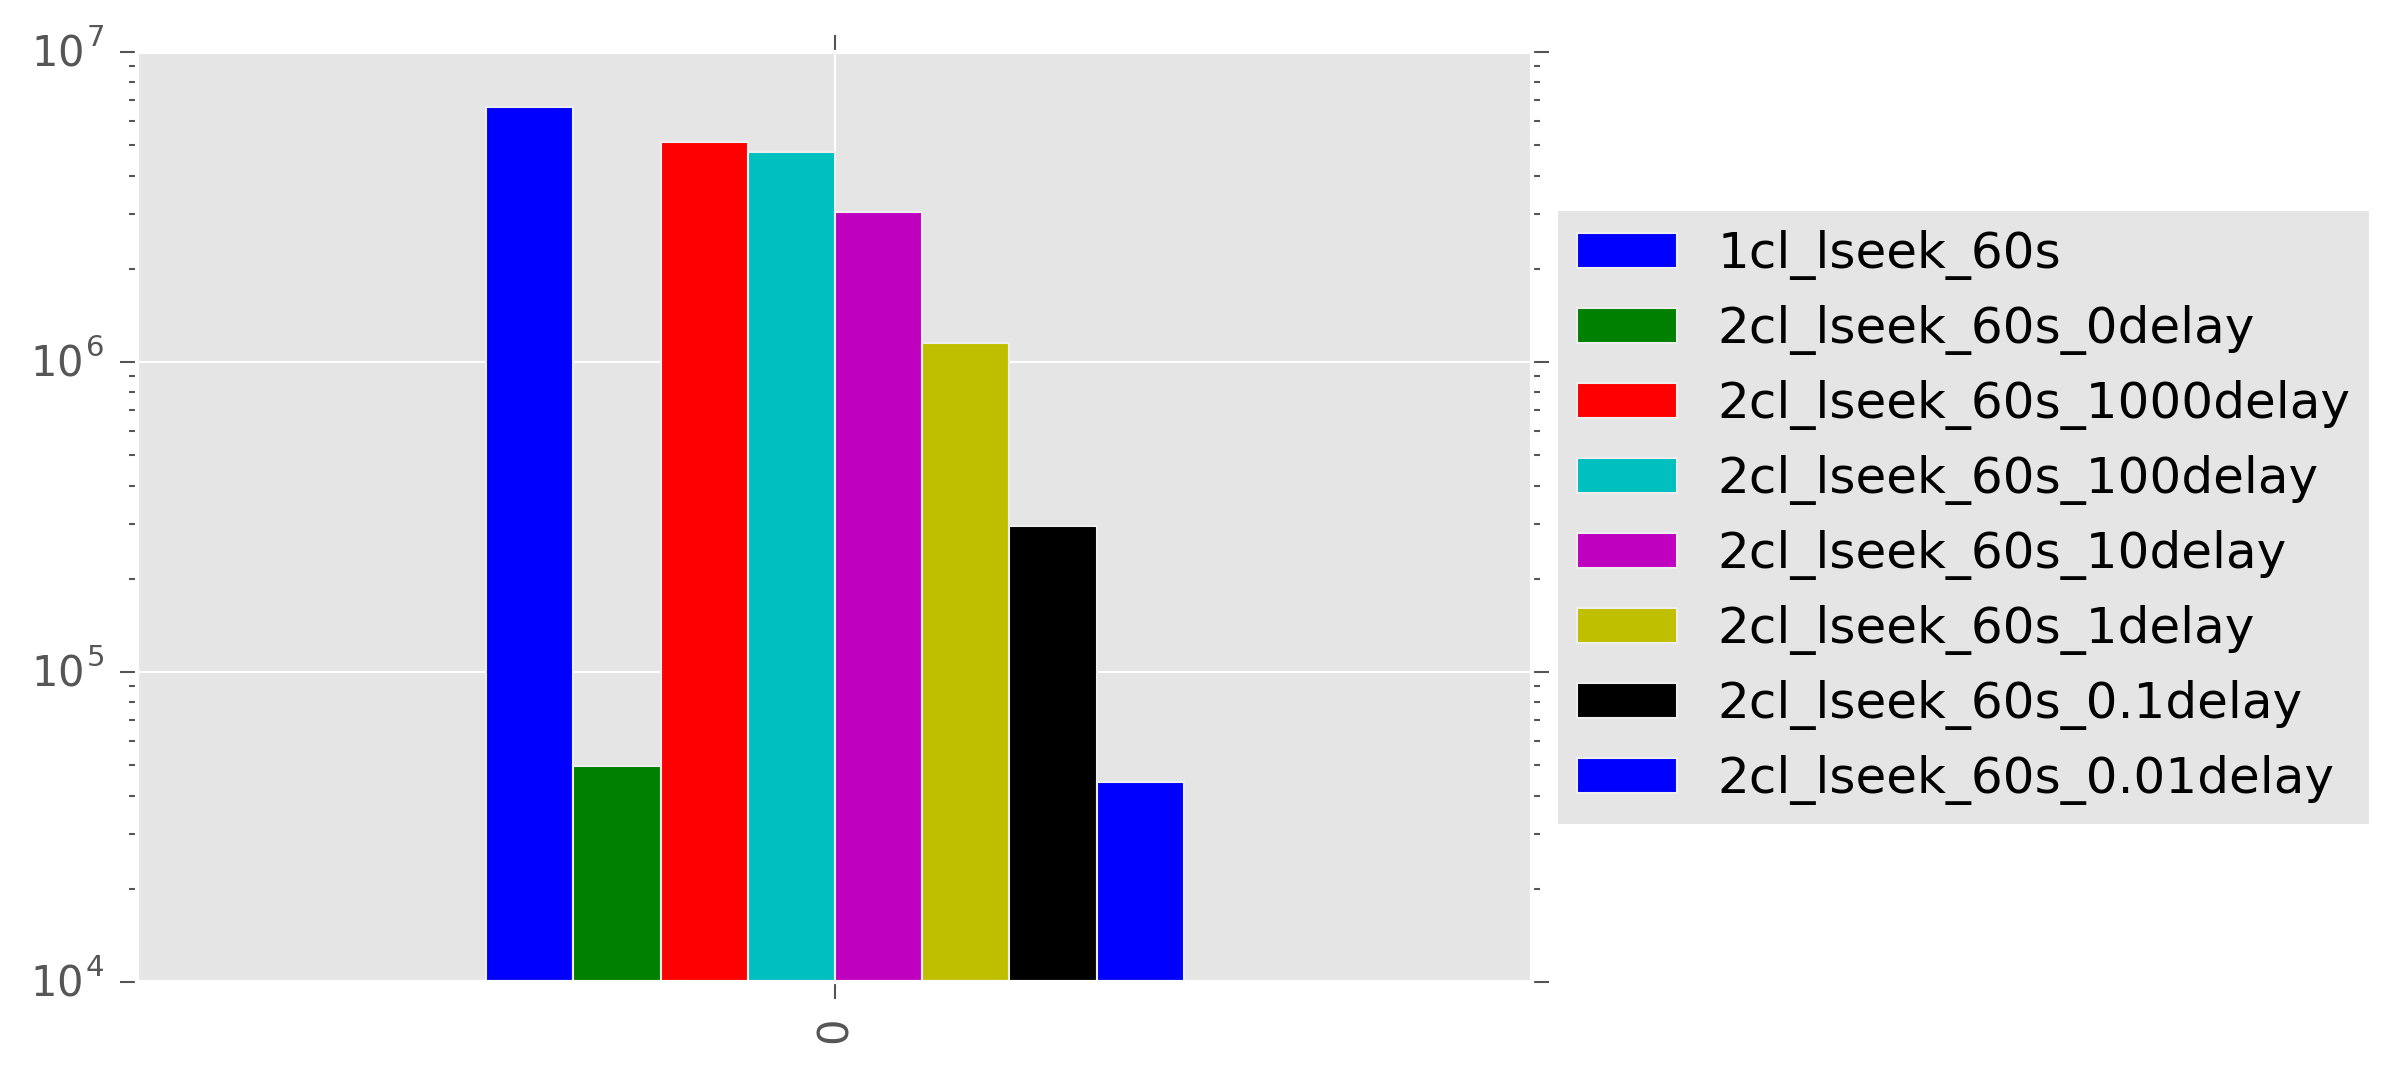
\includegraphics{figures/caps-delay-thruput.png}
\caption{Forcing the client to drop their capabilities later (delay)
improves throughput}
\end{figure}

\begin{figure}[htbp]
\centering
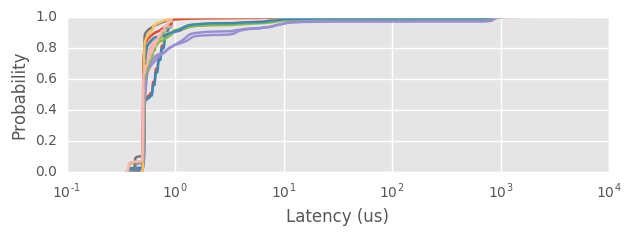
\includegraphics{figures/caps-delay-latency.png}
\caption{But if the clients hold their capabilities longer, it hurts
latency for everyone.}
\end{figure}

\subsubsection{CUT THIS Experiment: Client v. MDS caps +
Failures}\label{cut-this-experiment-client-v.-mds-caps-failures}

\subsubsection{Experiment: Mantle Sequencer
Balancer}\label{experiment-mantle-sequencer-balancer}

\section{Conclusion and Future Work}\label{conclusion-and-future-work}

Programmable storage is a viable method for eliminating duplication of
complex error prone software that are used as workarounds for storage
system deficiencies. However, this duplication has real-world problems
related to reliability. We propose that system expose their services in
a safe way allowing application developers to customize system behavior
to meet their needs while not sacrificing correctness.

We are intend to pursue this work towards the goal of constructing a set
of customization points that allow a wide variety of storage system
services to be configured on-the-fly in existing systems. This work is
one point along that path in which we have looked an a target
special-purpose storage system. Ultimately we want to utilize
declarative methods for expressing new services.

In conclusion, this paper should be accepted.

\bibliography{paper}
\bibliographystyle{plain}
%\printbibliography

\end{document}
